\chapter{Нейронна мережа як складова імпульсного радіоприймача}
\label{ch:neuron}

%%%%%%%%%%%%%%%%%%%%%%%%%%%%%%%%%%%%%%%%%%%%%%%%%%%%%%%%%%%%%%%%%%%%%%%%%%%%%%%
\section{Імпульсне радіо на нейронній схемотехніці}

\textcolor{red}{TODO: Провести аналогію до image classification transfer 
learing}

\textcolor{red}{TODO: поравняти методи навчання NLP з DeepUWB}

Імпульсні радіо-системи мають теоретичні переваги над вузькосмуговими, 
але на даний момент у імпульсних радіоприймачів виявлено ряд недоліків, 
через що їх практичне застосування обмежене або зовсім не доцільне. 
Використання нейронних мереж в якості апаратних кіл аналогової обробки 
дозволяє досягти більш якісного приймання та обробки сигналу ніж з 
існуючими засобами цифрової обробки прийнятого сигналу з антени.

Існуючі схеми імпульсних радіоприймачів передбачають послідовне надсилання 
та фільтрацію сигналу з антени лінійними пристроями, його оцифрування за 
допомогою аналого-цифрового перетворювача (АЦП) та класифікацію отриманого 
сигналу за його амплітудою та тривалістю. Тобто, розпізнається не сам сигнал, 
а його цифрова модель.

Таким чином, ефективність таких пристроїв обмежена порівняно невеликою 
частотою сканування  АЦП. Також, варто враховувати, що частина інформації 
з прийнятого сигналу губиться при фільтрації та квазілінійному підсиленні.

Послідовна аналогова та цифрова обробка для класифікації губить частину 
інформації про сигнал та про шум, що за визначенням погіршує якість 
класифікації. Такого не можна сказати про якісно навчену нейронну мережу, 
яка здатна виконувати таку саму функцію. З практики відомо, що 
найефективнішим методом класифікації є машинне навчання, отже доцільним 
було б застосувати нейронну мережу в якості модулю обробки прийнятого 
сигналу. 

Задачею імпульсного радіоприймача є перетворення в реальному часі сигналу 
з антени (часової послідовності) в деяку послідовність корисних даних. 
Для такої задачі гарно підходять рекурентні нейронні мережі, які накопичують 
інформацію про сигнал з плином часу та мають змогу до глибокого аналізу шуму 
та сторонніх сигналів, що підвищує якість роботи приймача.

Запропонований винахід принципово відрізняється від прототипів шляхом 
виділення корисної інформації з прийнятого сигналу. В основу існуючих 
пристроїв покладено принцип послідовного оцифрування та обробки, коли запропонована схема не потребує оцифрування сигналу для його обробки 
методами машинного навчання.

Необхідний винахідницький рівень в даному патенті досягається оцінкою 
технічних характеристик винаходу, оцінкою екологічних показників при 
поширеному застосуванні цієї технології та наявністю декількох схем 
аналогічних пристроїв для гнучкого запровадження виробництва  та наукових 
досліджень. Також  була проведена оцінка можливостей сучасної радіотехніки 
і електроніки для реалізації цього пристрою.

Даний винахід, на відміну від класичного приймача, має теоретичну змогу 
на автоматичне відокремлення сигналу від його перевідбиттів (луни) про що 
свідчать дослідження в сфері обробки мовлення. Зазначимо, що задача обробки 
мовлення та імпульсного сингалу розв’язуються однаково, а отже всі підходи 
до обробки мовлення можуть застосовуватись для обробки імпульсного сигналу. 

Для роботи класичних пристроїв необхідне стробоскопічне накопичування 
імпульсів для якісного оцифрування сигналу. При використанні нейронної 
схемотехніки пристрої АЦП не використовуються, а отже в необхідність в 
накопичуванні інформації про сигнал відпадає. Це дозволяє в рази підвищити 
інформаційну ємність імпульсного радіоканалу.

Нейронний процесор може бути перепрограмований, шляхом встановлення нових
параметрів нейронів, що дає змогу змінювати технічні характеристики 
пристроїв без їх заміни, що є більш екологічним та логістично вигідним.
Як і класична схема імпульсного радіо, запропонована схема передбачає 
можливість застосовувати одну і ту ж антену для передачі та прийму сигналу. 
Нейронний процесор повертає бінарний код отриманий з сигналу, а отже логіка 
його обробки не потребує складних на енерговитратних модулів FPGA, що 
робить приймальний пристрій більш привабливим для систем інтернету речей. 
За іншими показниками робота класичних пристроїв приймання імпульсного нестаціонарного радіосигналу повністю ідентична запропонованої, що 
дозволяє інтегрувати винахід до існуючих систем імпульсного 
радіомовлення та радіолокації.

\begin{figure}[htbp] \begin{center}
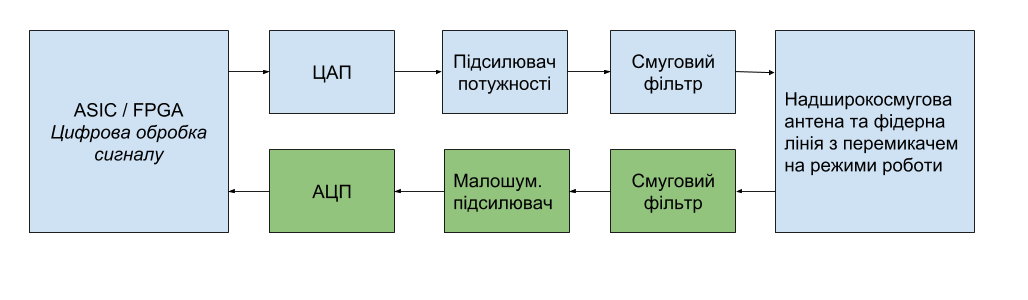
\includegraphics[scale=0.45]{classical_radio}
\caption{Класична схема імпульсного радіо} \label{fig:emp_radio}
\end{center} \end{figure}

Для поліпшення аналізу вхідних даних нейронною мережею пропонується 
сигнал з приймальної антени передавати з затримками, що дозволяє 
аналізувати не окреме значення амплітуди сигналу, а вікно у часі. 
Вікно вхідних даних передається на вхідний шар апаратної нейронної мережі. 
З'єднання нейронів необхідно виконати так, щоб дані обробки одно вікна 
переміщувались між шарами нейронної мережі одночасно. 

В якості додаткових, але не обов'язкових модулів передбачається стороннє 
живлення, пристрої підсилення та фіьтрації вхідного сигналу та шина зв'язку 
з драйвером пристрою, який дозволяє встановлювати або оновлювати параметри 
системи та отримувати інформацію про стан та налаштування пристрою.

Схема пристрою на Рис. 3 є найпростішим варіантом реалізації 
запропонованої технології. Обробка сигналу здійснюється нейронною 
мережею з одним внутрішнім шаром та малою кількістю нейронів. Розмір 
вхідного шару визначається кількістю елементів затримки та тривалістю 
вікна спостереження за сигналом. На виході з радіоприймального приладу 
отримаємо вектор бінарних значень, що описує приналежність сигналу у 
відповідному вікні спостереження до збудження одного чи іншого типу чи 
взагалі про відсутність сигналу. 

Для задач телекомунікації вихідний шар мережі виконується з персептронів. 
Тобто вихідний сигнал є бінарним сигналом, що може бути оброблений на 
вбудовувальній системі (embedded system) або системою на чіпі (SoC) 
під керування операційної системи. Розмір вихідного шару визначається 
кількістю сигналів, що необхідно розрізняти. При розпізнаванні більше 
ніж одного типу сигналів, схема обов'язково потребує нейрону 
відповідального за відсутність сигналу у вхідному шарі 
(вихід s0 на Рис. 3).

\begin{figure}[htbp] \begin{center}
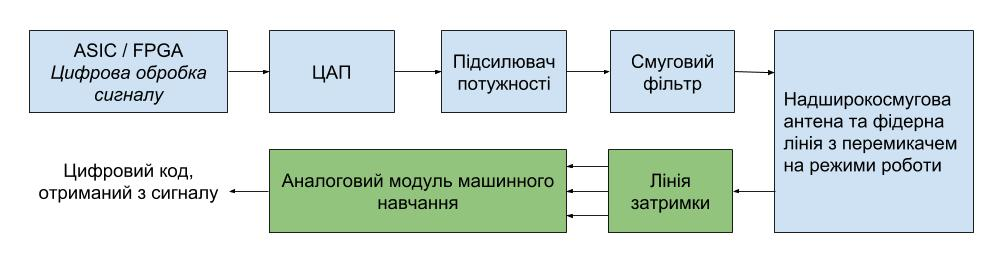
\includegraphics[scale=0.45]{neuron_radio}
\caption{Схема імпульсного радіо на нейронній схемотехніці} 
\label{fig:neural_radio}
\end{center} \end{figure}

На Рис. 3 використовуються два типи нейронів: персептрони 
(штучні нейрони вихідного шару) та штучні нейрони з сигмоідальною 
активацією (нейроноподібні елеметни вхідного шару). Використання саме 
таких видів нейроноподібних пристроїв не є оптимальним для класифікації 
та було вибрано для зручності електротехнічного виробництва. Станом на 
подання патентної заяви еквівалентні схеми даних штучних нейронів вже 
існують, а тому не приводяться в патенті.

Для досягнення універсальності виробничих ліній пропонується вбудовувати 
до елементів мережі більше штучних нейронів ніж необхідно. Також 
передбачається можливість перепрограмування кількості активних ліній 
затримки та їх характеристик. Такий підхід до організації налаштувань 
радіоприймача дозволить проводити програмне оновлення та зміну цільового 
призначення пристрою без зміни його апаратних складових.  Перед усім стає 
можливим оновлення протоколу імпульсної телекомунікації в залежності від 
умов навколишнього середовища та перенавчання нейронної мережі для різних 
форм збуджуючого імпульсу.

Дослідження показують, що пристрій на Рис. 3 не підходить для радарних 
задач. Це не єдина платня за простоту схеми - подана схема має низьку 
здатність до розрізнення накладених сигналів тому, особливо не має 
переваг перед класичним імпульсним радіо, але є привабливим для 
використання зразком при ведення наукової роботи та запровадження 
виробництва.

\begin{figure}[htbp] \begin{center}
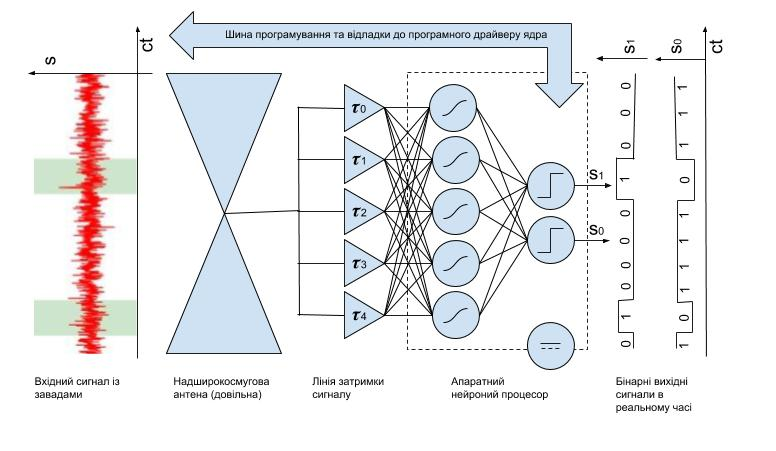
\includegraphics[scale=0.65]{simple_radio}
\caption{Імпульсне радіо на основі багатошарового персептрону} 
\label{fig:mp_radio}
\end{center} \end{figure}

Для використання всіх переваг винаходу необхідно ускладнити принцип 
роботи вбудованої нейронної мережі на Рис. 3. Перед усім, досвід 
машинного навчання в сфері обробки часових послідовностей стверджує що, 
доцільніше аналізувати не сигнал а його числові характеристики. 
Самі характеристики можуть бути різними та визначатись довільно. 
Головна вимога до набору параметрів, які описують сигнал - вони повинні 
однозначно вирізняти всі сигнали, що можуть бути прийняті антенною 
системою. В якості таких параметрів пропонується використовувати 
апаратне MFCC перетворення або деяку систему зі штучних нейронів, 
яка визначить набір параметрів автоматично. Не рекомендується 
використовувати різні евристичні та статистичні числові 
характеристики в якості параметрів сигналу.

Перед перетворенням сигналу на набір властивостей може використовуватись 
нейронна мережа зниження рівня шумів denoising autoencoder (NDA), 
яка покращить співвідношення сигналу до шуму. Для покращення роботи 
NDA можна накопичити минулі вікна спостереження, що додасть 
інформації про шум.

Схема на Рис. 4 показує, універсальну схему імпульсного радіо на 
нейронній схемотехніці. Універсальність досягається аналізом не самого 
сигналу, а його властивостей отриманих відповідним модулем, що дозволяє 
застосовувати методологію переносу навчання. Ця методологія дозволяє 
змінювати цільове призначення пристрою заміною або перенавчанням 
вихідного шару штучної нейронної системи.

Схеми на Рис. 3 і 4 не виключають застосування модулів аналогової 
обробки прийнятого сигналу, як на Рис. 1: лінійні фільтри 
та підсилювачі.

Даний винахід розширює область застосування імпульсного радіо за 
рахунок покращених робочих характеристик. Підвищена стійкість до 
шуму дозволяє вирішувати радарні та телекомунікаційні задачі на 
більших відстанях. Можливість розпізнавати імпульси різної форми 
збудження уможливлює кодування корисного сигналу імпульсами різної форми, 
що підвищує швидкість передачі даних. Також, відсутність класичного АЦП 
підвищує інформаційну ємність каналу, за рахунок відсутності 
стробоскопічних повторювань імпульсів для відтворення форми сигналу.

\begin{figure}[htbp] \begin{center}
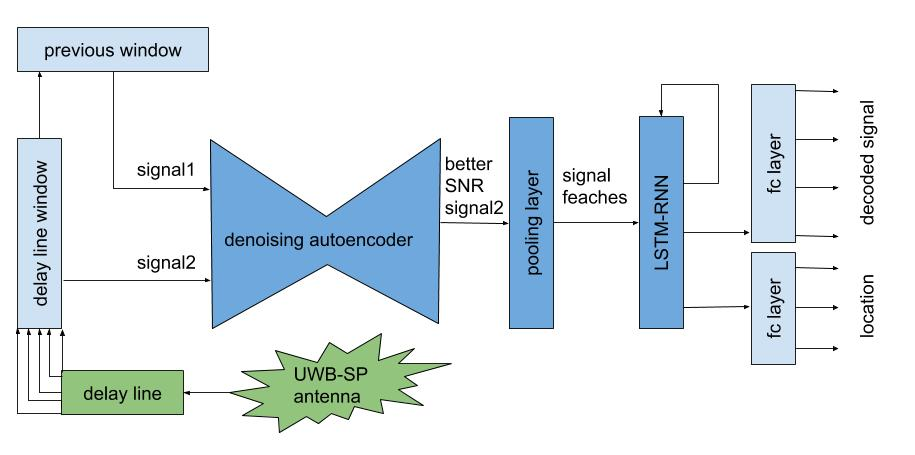
\includegraphics[scale=0.45]{netarch}
\caption{Імпульсне радіо на основі рекурентної нейронної мережі} 
\label{fig:rnn_radio}
\end{center} \end{figure}

Використання методології переносу навчання підвищує гнучкість 
застосування пристрою. Один і той самий прилад можна застосовувати для 
телекомунікаційних та радарних задач, встановленням різних 
конфігурацій на штучні нейрони та лінії затримки через шину 
програмування. Також, LSTM враховує і час приходу сигналу і його форму, 
що дозволяє одночасно вирішувати радарну задачу та задачу дистанційного 
зондування одним приладом.

%%%%%%%%%%%%%%%%%%%%%%%%%%%%%%%%%%%%%%%%%%%%%%%%%%%%%%%%%%%%%%%%%%%%%%%%%%%%%%%
\section{Переваги нейронної мережі, як засобу розвязання задач телекомунікації}

\begin{figure}[htbp] \begin{center}
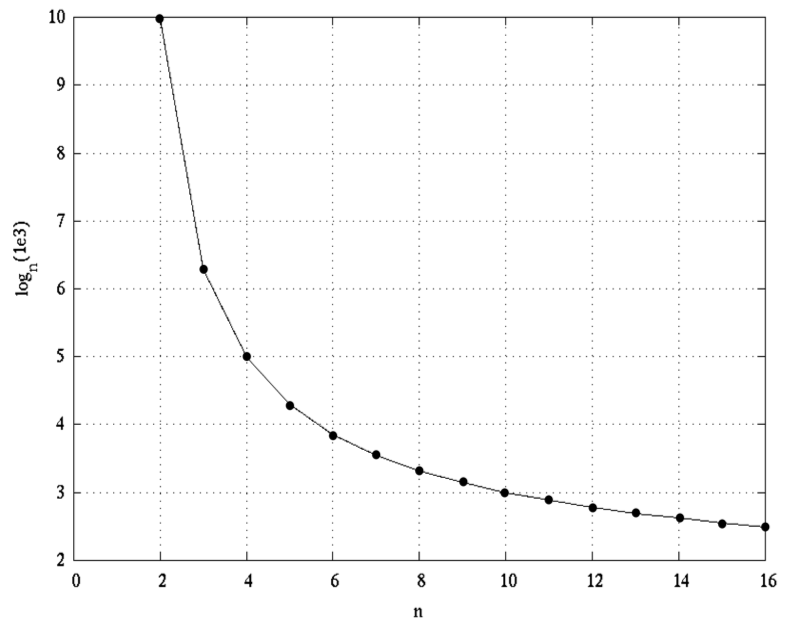
\includegraphics[scale=0.7]{channel_capacity}
\caption{Інформаційна емність імпульсного випромінювання} \label{fig:info_cap}
\end{center} \end{figure}

\begin{equation}
C = \frac{1}{N_{smp}} \frac{\log_2 \left( 1 + SNR \right)}{1/B + \tau_{RMS}} 
\end{equation}

%%%%%%%%%%%%%%%%%%%%%%%%%%%%%%%%%%%%%%%%%%%%%%%%%%%%%%%%%%%%%%%%%%%%%%%%%%%%%%%
\section{Оцінка стійкості апаратних нейронних мереж до шумів}

Розповсюдження сигналу через 

%%%%%%%%%%%%%%%%%%%%%%%%%%%%%%%%%%%%%%%%%%%%%%%%%%%%%%%%%%%%%%%%%%%%%%%%%%%%%%%
\section{Задача визначення кута за формую імпульсу}

Станом на сьогодні зокалізація за допомогою надширокосмугових імпульсних 
системвідбувається через вимірювання часу надходження відбитого 
випромінювання.

Використання нейроної мережі дозволить підвищіти точність такого 
вимірювання через визначення не тільки часу, а і азимутального 
кута прийому.

Для цього навчемо нейронну мережу розпізнавати кут за формою 
імпульсу, яка залежить від точки спостереження.

%%%%%%%%%%%%%%%%%%%%%%%%%%%%%%%%%%%%%%%%%%%%%%%%%%%%%%%%%%%%%%%%%%%%%%%%%%%%%%%
\section{Задача классифікації імпульсу в лінійному просторі}

%%%%%%%%%%%%%%%%%%%%%%%%%%%%%%%%%%%%%%%%%%%%%%%%%%%%%%%%%%%%%%%%%%%%%%%%%%%%%%%
\section{Задача классифікації імпульсу в нелінійному просторі}

%%%%%%%%%%%%%%%%%%%%%%%%%%%%%%%%%%%%%%%%%%%%%%%%%%%%%%%%%%%%%%%%%%%%%%%%%%%%%%%
\section{Задача клвсифікації в умовах детермінованого шуму}

%%%%%%%%%%%%%%%%%%%%%%%%%%%%%%%%%%%%%%%%%%%%%%%%%%%%%%%%%%%%%%%%%%%%%%%%%%%%%%%
\section{Радарна задача з системою антен типу LIRA та багатосмговою LSTM}
